\documentclass[border=0pt, multi, tikz]{standalone}
\usepackage{import}
\usepackage{amsmath,amssymb,amsfonts}
\usepackage[dvipsnames]{xcolor}

\subimport{./layers/}{init}
\usetikzlibrary{positioning}
\usetikzlibrary{3d}
\usetikzlibrary{calc}

\def\ConvColor{rgb:yellow,5;red,2.5;white,5}
\def\ConvReluColor{rgb:yellow,5;red,5;white,5}
\def\ConvSigmoidColor{rgb:yellow,5;red,7.5;white,5}
\def\PoolColor{rgb:red,1;black,0.3}
\def\DcnvColor{rgb:blue,5;green,2.5;white,5}
\def\SoftmaxColor{rgb:magenta,5;black,7}
\def\SumColor{rgb:red,5;purple,15;black,2.5}
\def\DiscColor{rgb:blue,5;green,15;black,8}
\def\MulColor{rgb:yellow,5;orange,15;black,8}
\def\ConcatColor{rgb:blue,5;red,2.5;white,5}
\def\FeatColor{rgb:gray,1}
\def\poolsep{1}

\begin{document}

\begin{tikzpicture}[
    > = {Latex[length=8, width=6]},
    pred/.style={
        draw, rounded corners=4px, fill=cyan!18, minimum width=78px, minimum height=69px, align=center},
    unk/.style={
        draw, rounded corners=4px, fill=gray!18, minimum width=78px, minimum height=69px, align=center},
    nodefeat/.style={
        draw, rounded corners=4px, fill=yellow!24, minimum width=78px, minimum height=35px, align=center},
    model/.style={
        draw, rounded corners=4px, fill=orange!16, minimum width=78px, minimum height=69px, align=center},
    Q/.style={
        draw, rounded corners=4px, fill=green!6, minimum width=78px, minimum height=69px, align=center},
    feat/.style={
        draw, rounded corners=4px, fill=yellow!24, minimum width=78px, minimum height=69px, align=center},
    io/.style={
        draw, rounded corners=4px, fill=violet!18, minimum width=78px, minimum height=69px, align=center},
    opr/.style={
        draw, rounded corners=0.5em, align=center
    },
]

\tikzset{arrow/.style={line width=1.25, draw={rgb:black,5}, rounded corners=4px}}

\fill[fill=gray!10] (-1-1.8-1, 0+2.3) rectangle (6.8+1.8+1, -9.6-2.0);
\fill[fill=gray!10] (19.2-1.8-1, 0+2.3) rectangle (23.3+0.2+1.8+1, -9.6-2.0);

\node[anchor=south] at (2.9, 1.6) {\scalebox{1.4}{\textbf{Pixel Domain}}};
\node[anchor=south] at (21.25, 1.6) {\scalebox{1.4}{\textbf{Superpixel Domain}}};

\node[io, arrow] at (-1, 0) (X) {
\includegraphics[width=72px,height=48px]{"./image.png"}\\ \scalebox{1.2}{$X$}};

\node[align=center, anchor=south] at (X.north) {\scalebox{1}{Input Image}};

\pic at ($(X.east) + (0.8, 0)$) {Box={
    name=mb0,
    fill=\ConvColor,
    height=8,
    width=0.075*16,
    depth=8
}};

\draw[->, arrow] (X) -- (mb0-west);

\pic at ($(mb0-east) + (0, 0)$) {RightBandedBox={
    name=mb1,
    fill=\ConvColor,
    bandfill=\ConvReluColor,
    height=8*0.5,
    width=0.075*16,
    depth=8*0.5
}};

\pic at ($(mb1-east) + (0, 0)$) {RightBandedBox={
    name=mb2,
    fill=\ConvColor,
    bandfill=\ConvReluColor,
    height=8*0.25,
    width=0.075*24,
    depth=8*0.25
}};

\pic at ($(mb2-east) + (0, 0)$) {RightBandedBox={
    name=mb3,
    fill=\ConvColor,
    bandfill=\ConvReluColor,
    height=8*0.125,
    width=0.075*40,
    depth=8*0.125
}};

\pic at ($(mb3-east) + (0, 0)$) {RightBandedBox={
    name=mb4,
    fill=\ConvColor,
    bandfill=\ConvReluColor,
    height=8*0.125,
    width=0.075*48,
    depth=8*0.125
}};

\pic at ($(mb4-east) + (0, 0)$) {RightBandedBox={
    name=mb5,
    fill=\ConvColor,
    bandfill=\ConvReluColor,
    height=8*0.0625,
    width=0.075*96,
    depth=8*0.0625
}};

\node[align=center] at ($(mb0-west)!0.5!(mb5-east) + (0, -0.8)$) {
    \scalebox{1}{CNN}\\
    \scalebox{1}{Backbone}
};

\node[feat, arrow] at (6.8, 0) (Fp) {
\includegraphics[width=72px,height=48px]{"./random-blue/random2d.pdf"}\\ \scalebox{1.2}{$F_p$}};

\draw[->, arrow] (mb5-east) -- (Fp.west);

\node[align=center, anchor=south] at (Fp.north) {\scalebox{1}{Pixel-Level Features}};

% \node[io, arrow] at (9.4, -3.2) (awa) {
\includegraphics[width=72px,height=48px]{"./image.png"}\\ \scalebox{1.2}{image}};

\pic at ($(X.center) + (1.1, -3)$) {Box={
    name=sfcn0,
    fill=\ConvColor,
    height=7,
    width=0.0375*16,
    depth=7
}};

\draw[->, arrow] (X) |- (sfcn0-west);

\pic at ($(sfcn0-east) + (0, 0)$) {Box={
    name=sfcn1,
    fill=\ConvColor,
    height=8*0.5,
    width=0.0375*32,
    depth=8*0.5
}};

\pic at ($(sfcn1-east) + (0, 0)$) {Box={
    name=sfcn2,
    fill=\ConvColor,
    height=8*0.25,
    width=0.0375*64,
    depth=8*0.25
}};

\pic at ($(sfcn2-east) + (0, 0)$) {Box={
    name=sfcn3,
    fill=\ConvColor,
    height=8*0.125,
    width=0.0375*128,
    depth=8*0.125
}};

\pic at ($(sfcn3-east) + (0, 0)$) {Box={
    name=sfcn4,
    fill=\ConvColor,
    height=8*0.0625,
    width=0.0375*256,
    depth=8*0.0625
}};

\pic at ($(sfcn4-east) + (0, 0)$) {Box={
    name=sfcn5,
    fill=\DcnvColor,
    height=8*0.125,
    width=0.0375*128,
    depth=8*0.125
}};

\draw[->, arrow] (sfcn3-east) |- ($(sfcn4-anchor) + (0, 0.3)$) -| (sfcn5-west);

\pic at ($(sfcn5-east) + (0, 0)$) {Box={
    name=sfcn6,
    fill=\DcnvColor,
    height=8*0.25,
    width=0.0375*64,
    depth=8*0.25
}};

\draw[->, arrow] (sfcn2-east) |- ($(sfcn4-anchor) + (0, 0.5)$) -| (sfcn6-west);

\pic at ($(sfcn6-east) + (0, 0)$) {Box={
    name=sfcn7,
    fill=\DcnvColor,
    height=8*0.5,
    width=0.0375*32,
    depth=8*0.5
}};

\draw[->, arrow] (sfcn1-east) |- ($(sfcn4-anchor) + (0, 0.8)$) -| (sfcn7-west);

\pic at ($(sfcn7-east) + (0, 0)$) {Box={
    name=sfcn8,
    fill=\DcnvColor,
    height=7,
    width=0.0375*16,
    depth=7
}};

\draw[->, arrow] (sfcn0-east) |- ($(sfcn4-anchor) + (0, 1.2)$) -| (sfcn8-west);

% \draw[->] ($(mb0-west)!0.5!(mb5-east)$) -| (sfcn4-anchor);

\node[] at ($(sfcn4-anchor) + (0, -0.5)$) {\scalebox{1}{SpixelFCN}};

\node[pred, arrow] at (-1, -6.4) (yhat) {
\includegraphics[width=72px,height=48px]{"./pred.png"}\\ \scalebox{1.2}{$\hat{Y}$}};

\node[align=center, anchor=south] at (yhat.north) {
    \scalebox{1}{Pixel-Wise Prediction}
};

\node[io, arrow] at (-1, -9.6) (gt) {
\includegraphics[width=72px,height=48px]{"./gt.png"}\\ \scalebox{1.2}{$Y$}};

\node[align=center, anchor=north] at (gt.south) {\scalebox{1}{Ground Truth}};

\draw[->, densely dashed, arrow] (yhat.south) -- (gt.north);

\node[anchor=west] at ($(yhat.south)!0.5!(gt.north) + (0.05, 0)$)
{\scalebox{1.}{$\mathcal{L}_{p}(\cdot)$}};

\coordinate (dec-west) at ($(yhat.east) + (1.2, 0.8)$);
\coordinate (dec-east) at ($(dec-west) + (2.5, 0)$);
\filldraw[fill=orange!16]
    ($(dec-west) + (0, 0.75)$)
    -- ($(dec-east) + (0, 1.25)$)
    -- ($(dec-east) + (0, -1.25)$)
    -- ($(dec-west) + (0, -0.75)$)
    -- cycle;
\draw[line width=0.75]
    ($(dec-west) + (0, 0.75)$)
    -- ($(dec-east) + (0, 1.25)$)
    -- ($(dec-east) + (0, -1.25)$)
    -- ($(dec-west) + (0, -0.75)$)
    -- cycle;
\node[align=center] at ($(dec-east)!0.5!(dec-west)$) {
    \scalebox{1}{Feature-Fusion}\\
    \scalebox{1}{Decoder}
};
\draw[->, arrow] (dec-west) -| ($(dec-west)!0.5!(yhat.east)$) |- (yhat.east);
\draw[->, arrow] (Fp.south) |- ($(dec-east) + (0, 0.5)$);

\node[feat, arrow] at (6.8, -6.4-1.3) (Fg) {
\includegraphics[width=72px,height=48px]{"./random-red/random2d.pdf"}\\ \scalebox{1.2}{$F_g$}};

\node[align=center, anchor=north] at (Fg.south) {
    \scalebox{1}{DisAggregated GNN Features}
};

\draw[->, arrow] (Fg.north) |- ($(dec-east) + (0, -0.3)$);

\node[Q, arrow] at (13, -3) (Q) {
\includegraphics[width=72px,height=48px]{"./random-black/random2d.pdf"}\\ \scalebox{1.2}{$Q$}};

\node[align=center, anchor=north] at ($(Q.south) + (0, -0.1)$) {
    \scalebox{0.9}{Pixel-to-Superpixel}\\
    \scalebox{1}{Affinity Matrix}
};

\draw[->, arrow] (sfcn8-east) -- (Q.west);

\node[opr, arrow] at (13, 0) (Fp2Fsp) {$\mathrm{Agg}_{Q}(\cdot)$};
\draw[arrow] (Fp.east) -- (Fp2Fsp.west);
\draw[->, arrow] (Q.north) -- (Fp2Fsp.south);


\node[opr, arrow] at (11, -6.4-1.3+0.6) (Fn2Fg) {$\mathrm{DisAgg}_{Q}(\cdot)$};
\draw[->, arrow] (Fn2Fg.west) -- ($(Fg.east) + (0, 0.6)$);
\draw[->, arrow] ($(Q.south west) + (0.05, 0.05)$) -- ++(-0.65,-0.65) -- (Fn2Fg.north);

\node[Q, arrow] at (19.2, -3) (G) {
\includegraphics[width=72px,height=48px]{"./graph-icon.png"}\\ \scalebox{1.2}{$G$}};
\node[align=center, anchor=south] at (G.north) {\scalebox{1}{Graph}};
\draw[->, arrow] (Q.east) -- (G.west);

\node[nodefeat, arrow] at (23.3, 0) (Fsp) {
\includegraphics[width=72px]{"./random1d-blue/random2d.pdf"}\\ \scalebox{1.2}{$F_{sp}$}};
\node[align=center, anchor=south] at (Fsp.north) {
    \scalebox{1}{Superpixel-Level Features}
};
\draw[->, arrow] (Fp2Fsp.east) -- (Fsp.west);

\node[model, arrow, minimum height=120, minimum width=95] at (23.3, -3.5) (GCN) {};

\node[anchor=south east] at ($(GCN.north east)$) {\scalebox{1}{GNN}};

\node[
    inner sep=0, outer sep=0,
    xslant=0.6,
    yslant=0.0,
    fill={rgb:white,5},
    opacity=1.,
    draw
  ] at ($(GCN.south) + (0, 1)$) (gcnn) {
    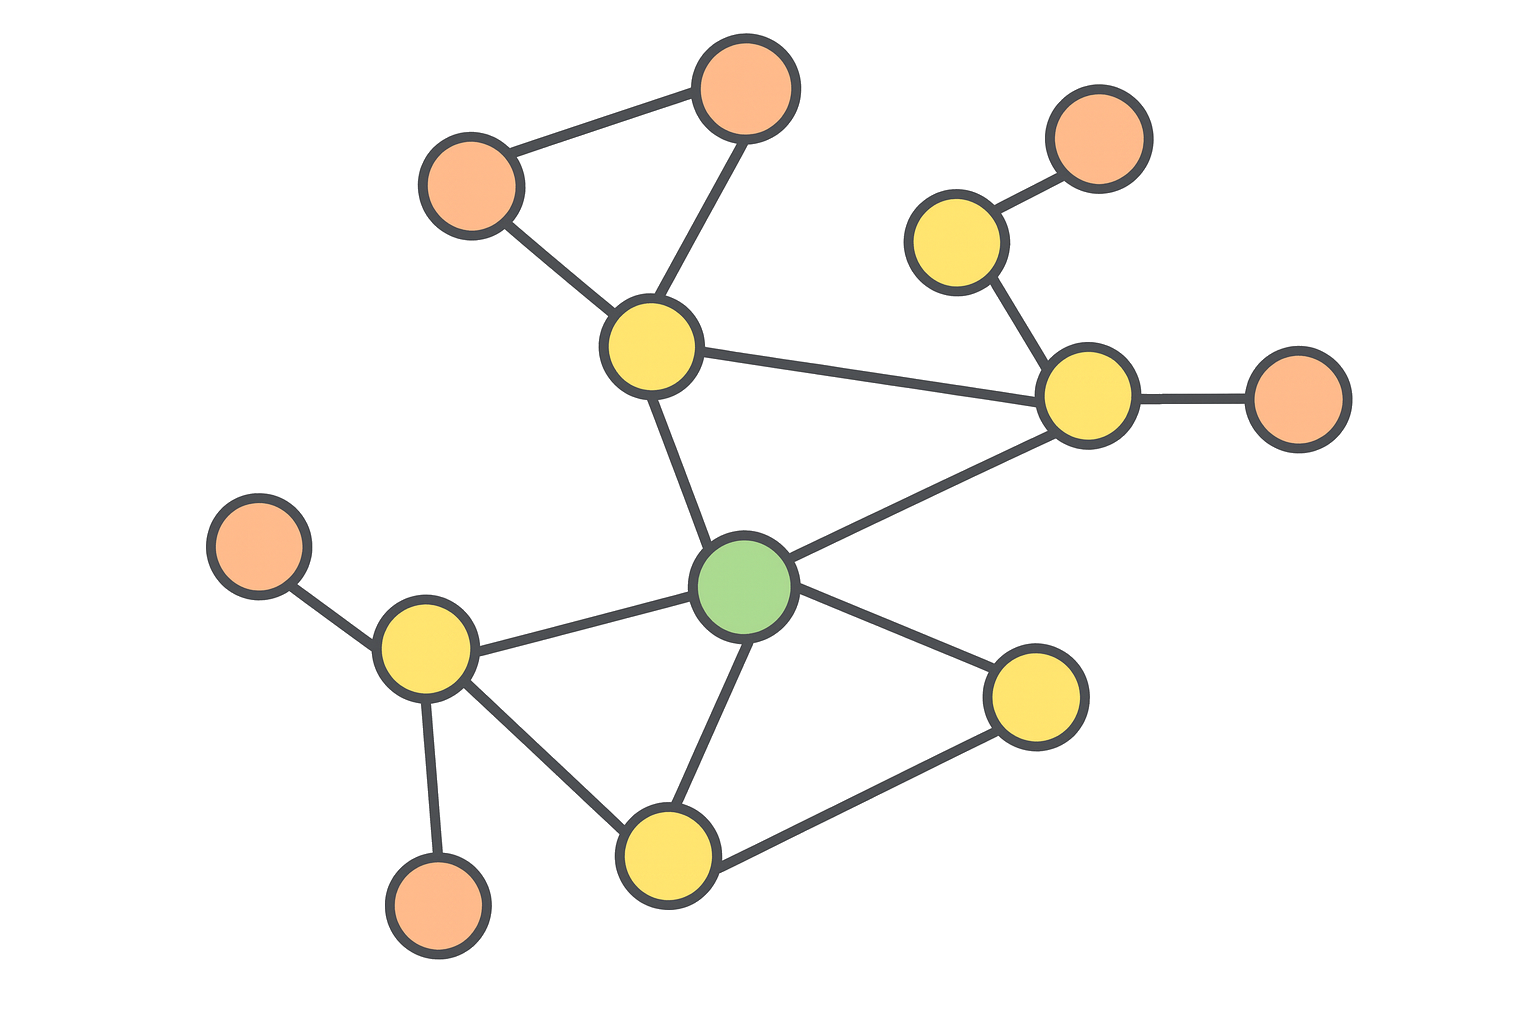
\includegraphics[width=60px, height=30px]{./graph-icon.png}
};
\node[
    inner sep=0, outer sep=0,
    xslant=0.6,
    yslant=0.0,
    fill={rgb:white,5},
    opacity=0.3,
    draw
  ] at ($(GCN.north) + (0, -2)$) (gcn5)
  {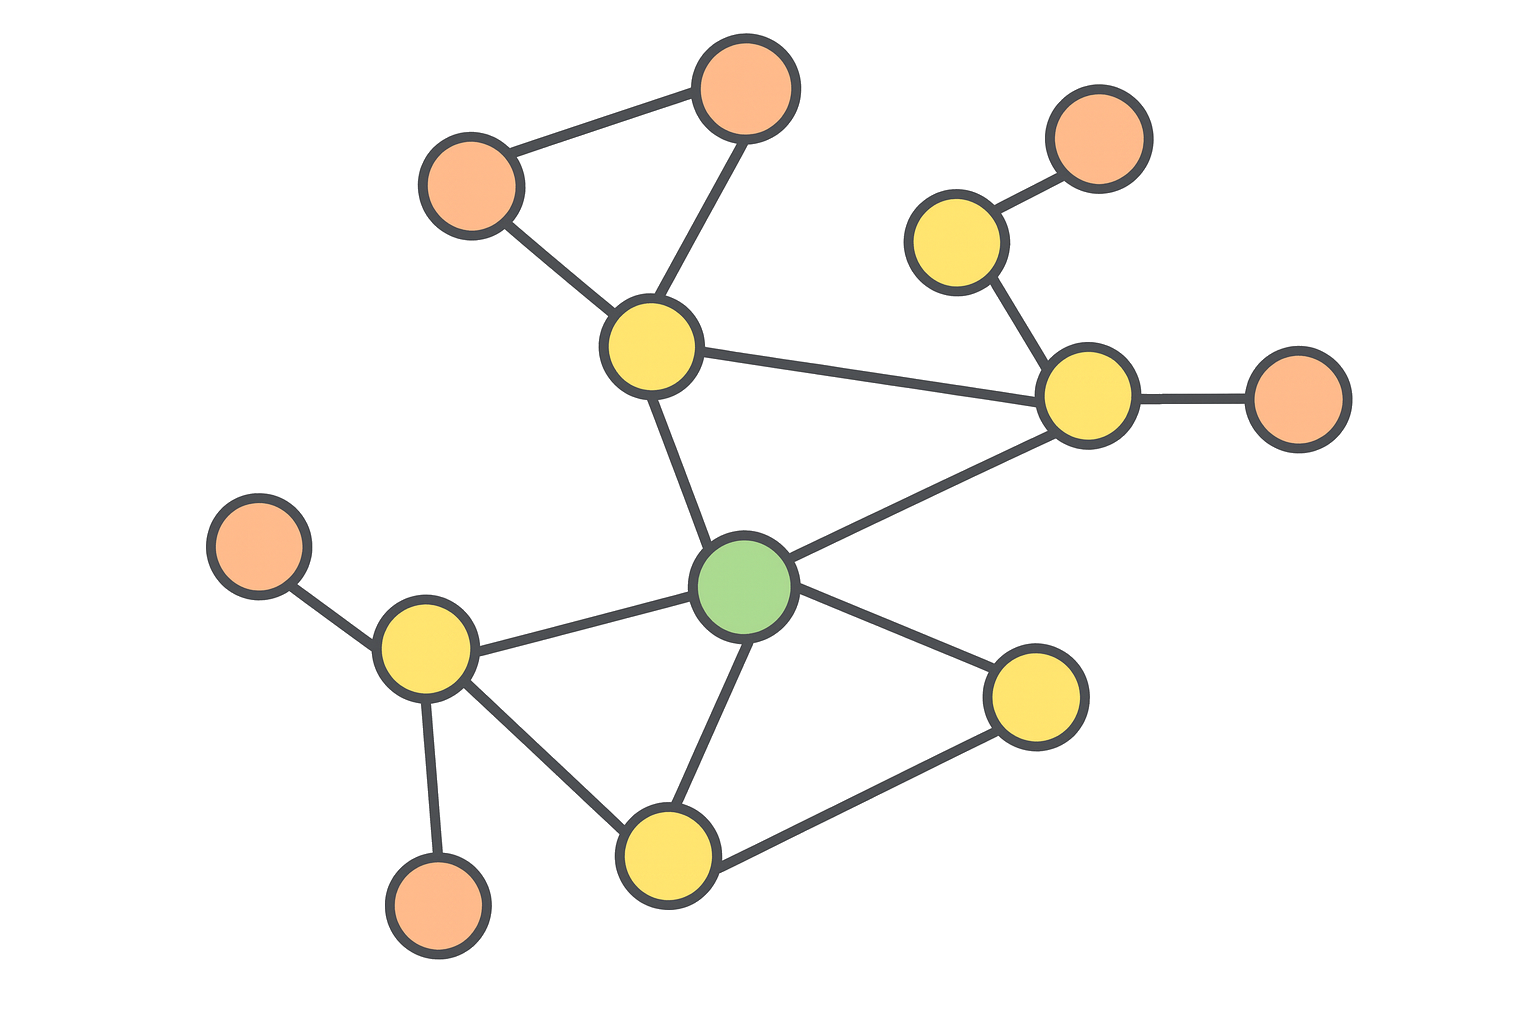
\includegraphics[width=60px, height=30px]{./graph-icon.png}};
\node[
    inner sep=0, outer sep=0,
    xslant=0.6,
    yslant=0.0,
    fill={rgb:white,5},
    opacity=0.6,
    draw
  ] at ($(gcn5.center) + (0, 0.25)$) (gcn4)
  {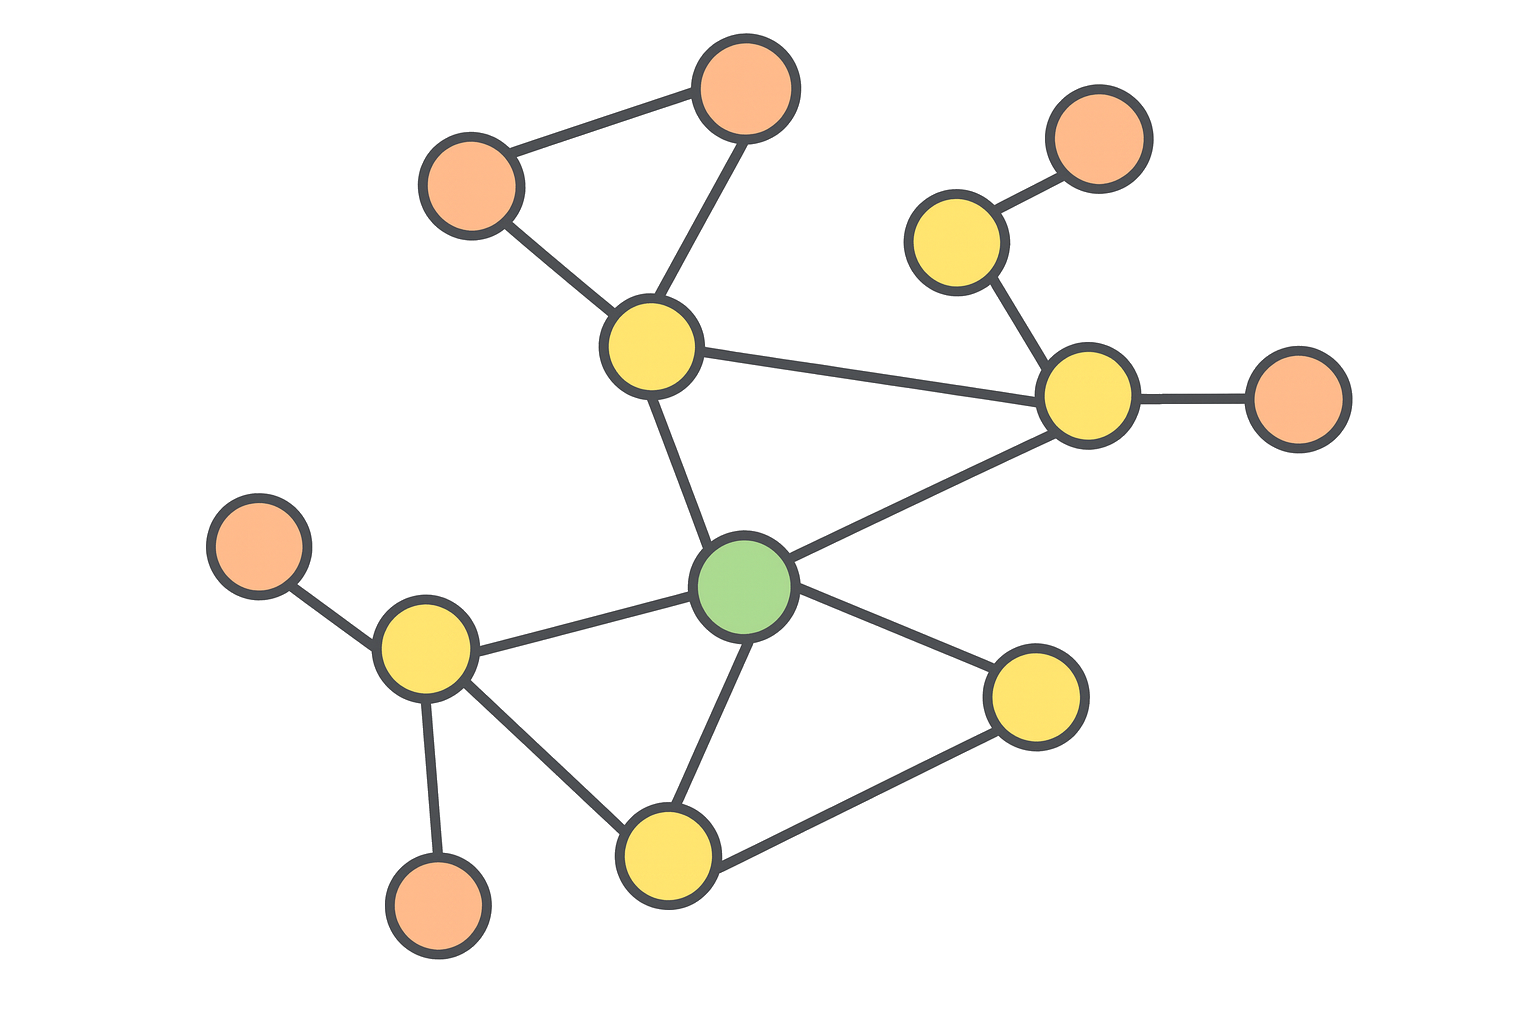
\includegraphics[width=60px, height=30px]{./graph-icon.png}};
\node[
    inner sep=0, outer sep=0,
    xslant=0.6,
    yslant=0.0,
    fill={rgb:white,5},
    opacity=0.9,
    draw
  ] at ($(gcn4.center) + (0, 0.25)$) (gcn3)
  {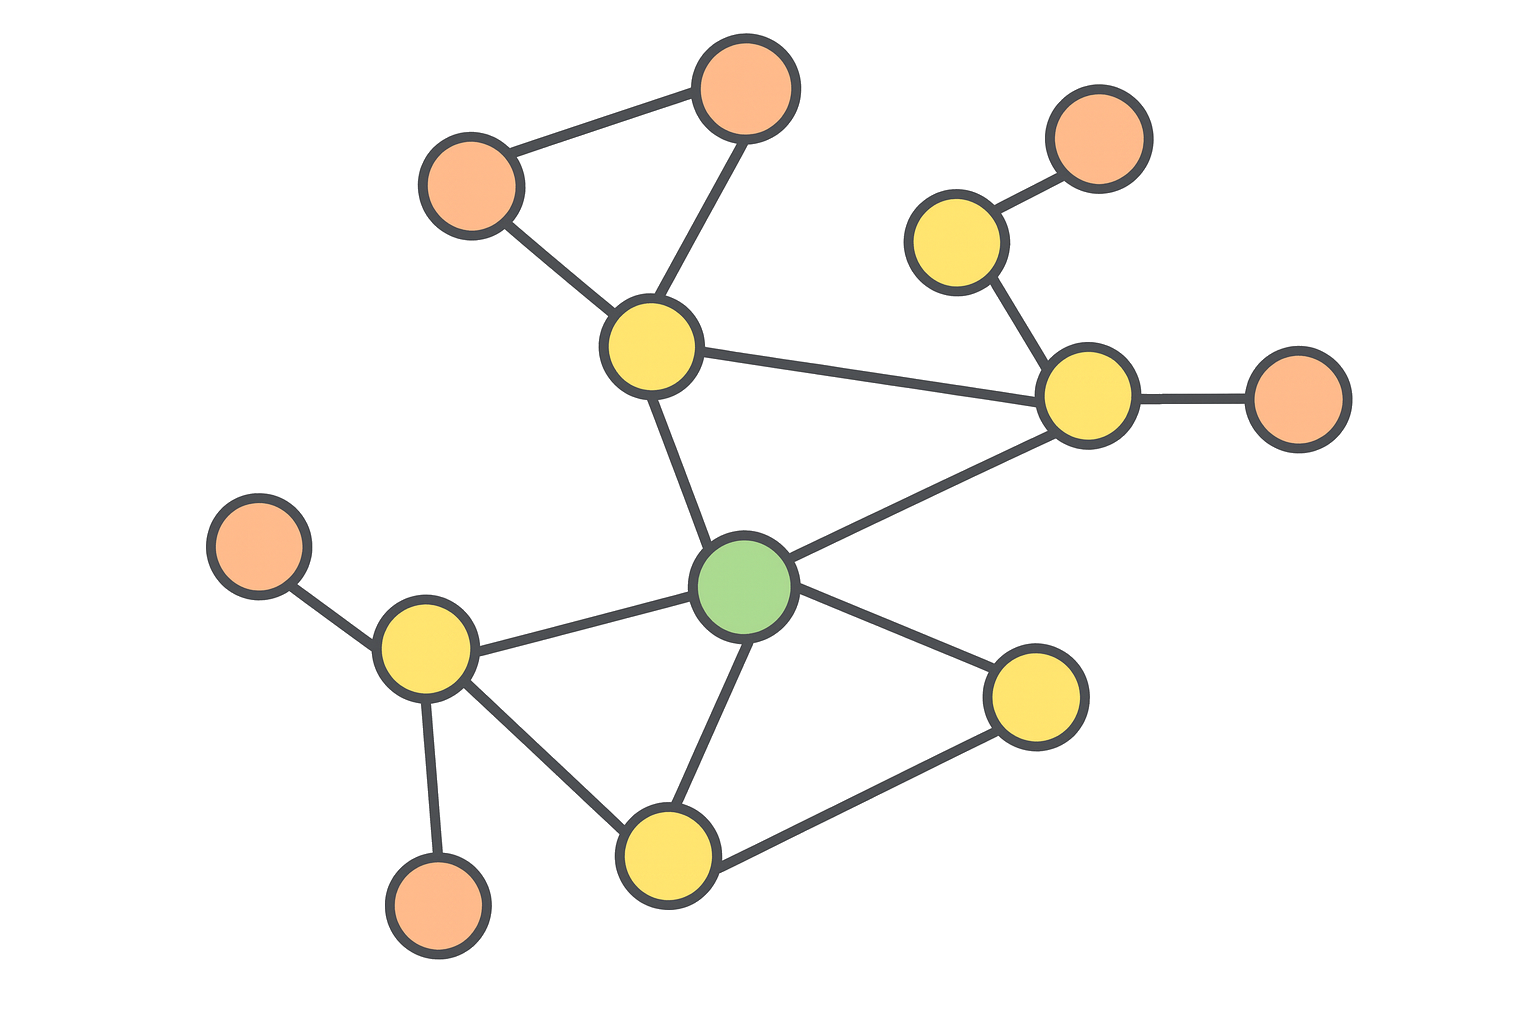
\includegraphics[width=60px, height=30px]{./graph-icon.png}};
\node[
    inner sep=0, outer sep=0,
    xslant=0.6,
    yslant=0.0,
    fill={rgb:white,5},
    opacity=1.,
    draw
  ] at ($(gcn3.center) + (0, 0.25)$) (gcn2)
  {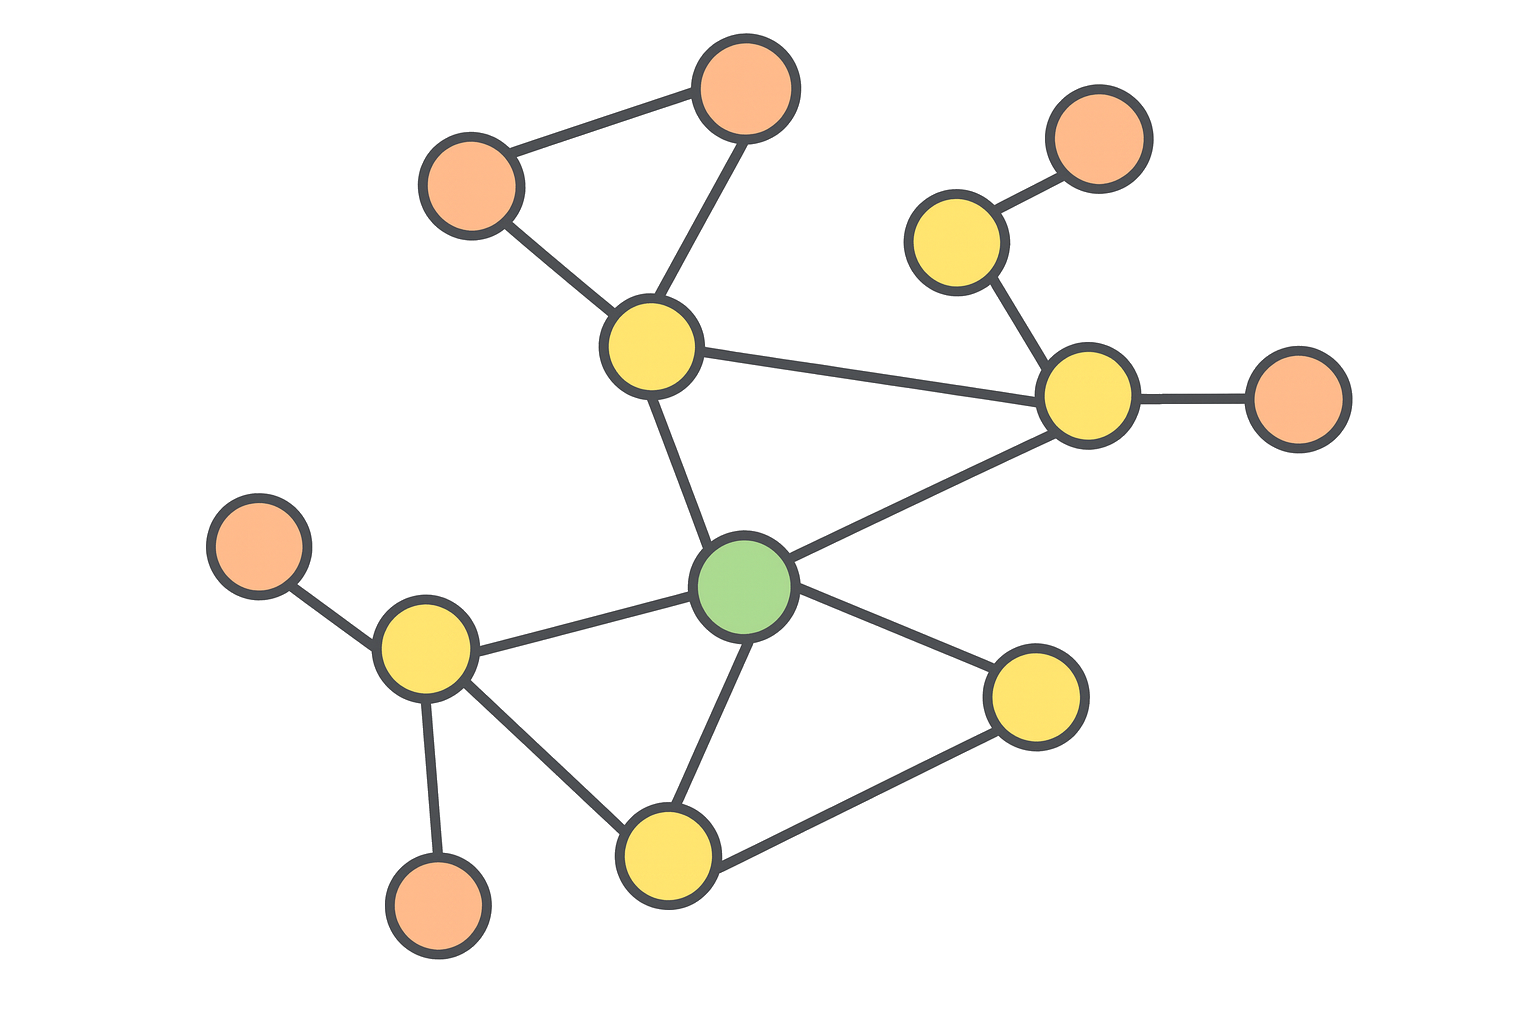
\includegraphics[width=60px, height=30px]{./graph-icon.png}};
\node[
    inner sep=0, outer sep=0,
    xslant=0.6,
    yslant=0.0,
    fill={rgb:white,5},
    opacity=1.,
    draw
  ] at ($(gcn2.center) + (0, 0.25)$) (gcn1)
  {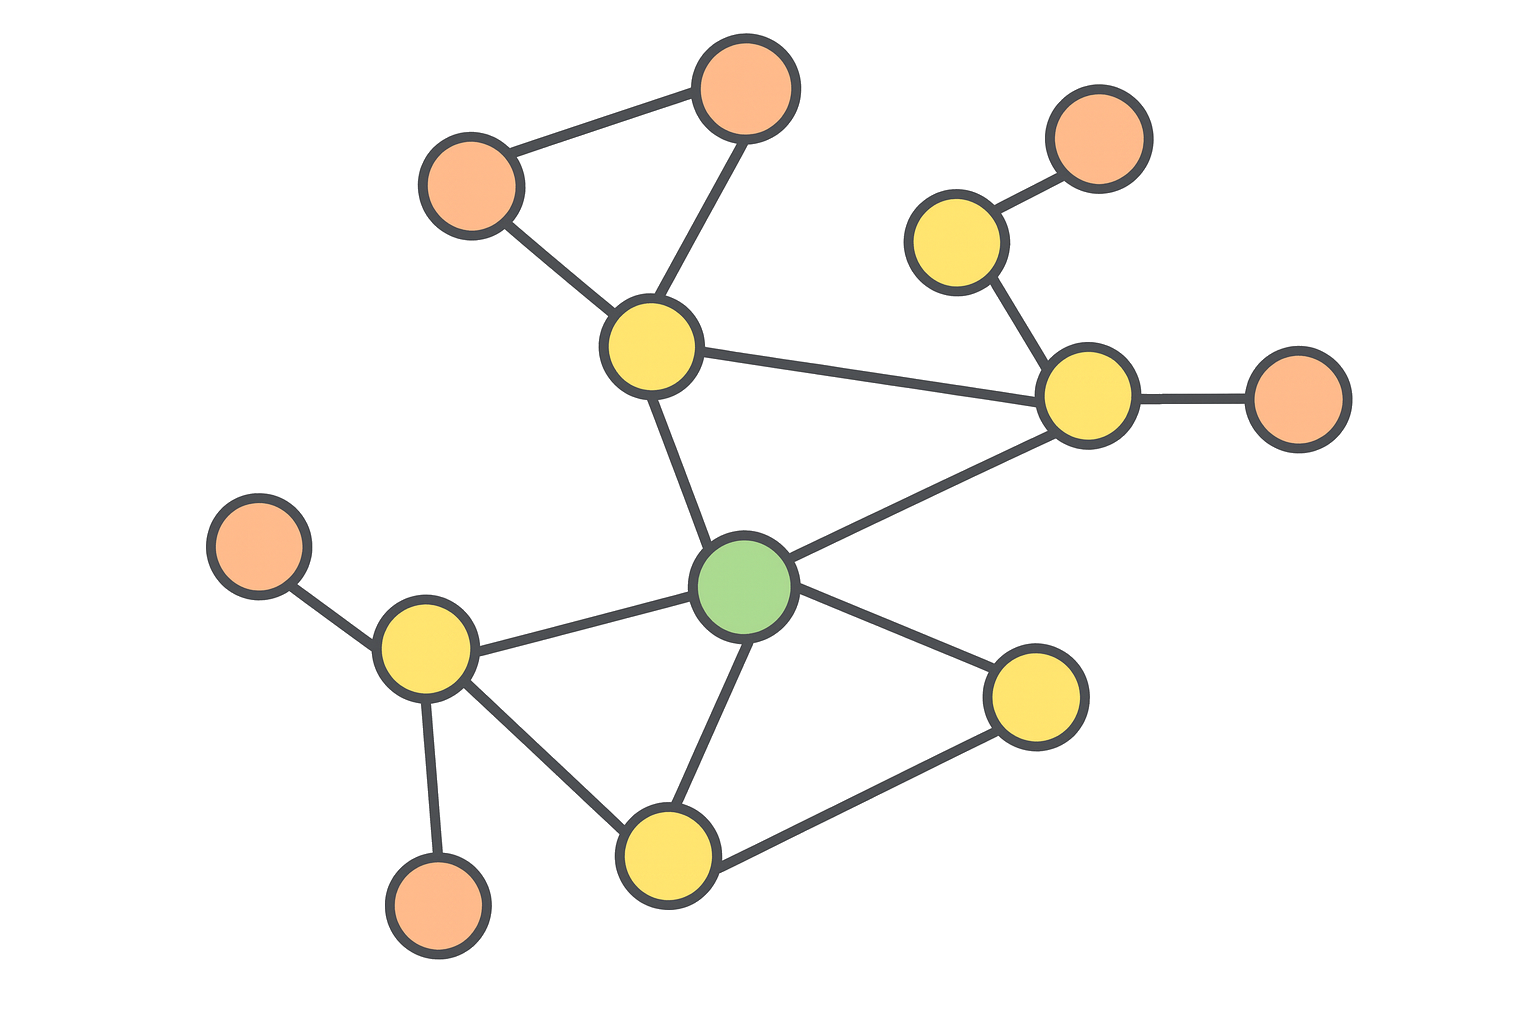
\includegraphics[width=60px, height=30px]{./graph-icon.png}};


\draw[->, arrow] (Fsp.south) -- ($(GCN.north) + (0, -1)$);
\draw[->, arrow] (G.east) -- ($(GCN.west) + (0, 0.5)$);

\node[nodefeat, arrow] at (23.3, -6.4-1.3+0.6) (Fn) {
\includegraphics[width=72px]{"./random1d-red/random2d.pdf"}\\ \scalebox{1.2}{$F_n$}};
\draw[->, arrow] ($(GCN.south) + (0, 0.47)$) -- (Fn.north);
\draw[arrow] (Fn.west) -- (Fn2Fg.east);

\node[pred, arrow] at (23.3, -9.6) (ysphat) {
\includegraphics[width=72px,height=48px]{"./pred-node.png"}\\ \scalebox{1.2}{$\hat{Y}_{sp}$}};
\node[align=center, anchor=north] at (ysphat.south) {\scalebox{1}{Node-Wise Prediction}};

\draw[->, arrow] (Fn.south) -- (ysphat.north);
\node[anchor=west] at ($(Fn.south)!0.5!(ysphat.north) + (0.05, 0)$)
{\scalebox{1.}{$\mathrm{FC}$}};

\node[opr, arrow] at (15, -9.6-0.6) (Y2Ysp) {$\mathrm{Agg}_{Q}(\cdot)$};
\draw[arrow] ($(gt.east) + (0, -0.6)$) -- (Y2Ysp.west);
\draw[->, arrow] ($(Q.south east) + (-0.05, 0.05)$) -- ++(0.65,-0.65) -- (Y2Ysp.north);

\node[io, arrow] at (19.2, -9.6) (Ysp) {
\includegraphics[width=72px,height=48px]{"./gt-node.png"}\\ \scalebox{1.2}{$Y_{sp}$}};
\node[align=center, anchor=south] at (Ysp.north) {
    \scalebox{1}{Class Distribution}\\
    \scalebox{1}{in Superpixels}
};
\draw[->, arrow] (Y2Ysp.east) -- ($(Ysp.west) + (0, -0.6)$);

\draw[->, densely dashed, arrow] ($(ysphat.west) + (0, -0.6)$) -- ($(Ysp.east) + (0, -0.6)$);
\node[anchor=south] at ($(ysphat.west)!0.5!(Ysp.east) + (0, -0.6+0.05)$)
{\scalebox{1.}{$\mathcal{L}_{sp}(\cdot)$}};

% grads

\tikzset{grad/.style={line width=1.25, draw={rgb:red,5}, rounded corners=4px}}

\draw[->, grad] ($(Ysp.east) + (0, -0.8)$) -- ($(ysphat.west) + (0, -0.8)$);

\draw[->, grad] ($(ysphat.north) + (-0.2, 0)$) -- ($(Fn.south) + (-0.2, 0)$);

\draw[->, grad] ($(Fn.north) + (-0.2, 0)$) -- ($(GCN.south) + (-0.2, 0.47)$);

\draw[->, grad] ($(GCN.north) + (-0.2, -1)$) -- ($(Fsp.south) + (-0.2, 0)$);

\draw[grad] ($(Fsp.west) + (0, -0.2)$) -- ($(Fp2Fsp.east) + (0, -0.2)$);

\draw[->, grad] ($(Fp2Fsp.west) + (0, -0.2)$) -- ($(Fp.east) + (0, -0.2)$);

\draw[->, grad] ($(Fp.west) + (0, -0.2)$) -- ($(mb5-east) + (0, -0.2)$);

\draw[->, grad] ($(Fp2Fsp.south) + (-0.2, 0)$) -- ($(Q.north) + (-0.2, 0)$);

\draw[->, grad] ($(Q.west) + (0, 0.2)$) -- ($(sfcn8-east) + (0, 0.2)$);

\draw[->, grad, rounded corners=2px] ($(dec-east) + (0, 0.5+0.2)$) -| ($(Fp.south) + (-0.2, 0)$);

\draw[->, grad, rounded corners=2px] ($(dec-east) + (0, -0.3-0.2)$) -| ($(Fg.north) + (-0.2, 0)$);

\draw[grad] ($(Fg.east) + (0, 0.2+0.6)$) -- ($(Fn2Fg.west) + (0, 0.2)$);

\draw[->, grad] ($(Fn2Fg.east) + (0, 0.2)$) -- ($(Fn.west) + (0, 0.2)$);

\draw[grad, rounded corners=6px] ($(yhat.east) + (0, -0.2)$) -| ($(dec-west)!0.5!(yhat.east) + (0.2, -0.2)$);

\draw[->, grad, rounded corners=2px] ($(dec-west)!0.5!(yhat.east) + (0.2, -0.2)$) |- ($(dec-west) + (0, -0.2)$);

\draw[->, grad] ($(gt.north) + (-0.2, 0)$) -- ($(yhat.south) + (-0.2, 0)$);

\end{tikzpicture}

\end{document}